% Options for packages loaded elsewhere
\PassOptionsToPackage{unicode}{hyperref}
\PassOptionsToPackage{hyphens}{url}
%
\documentclass[
]{article}
\usepackage{amsmath,amssymb}
\usepackage{lmodern}
\usepackage{ifxetex,ifluatex}
\ifnum 0\ifxetex 1\fi\ifluatex 1\fi=0 % if pdftex
  \usepackage[T1]{fontenc}
  \usepackage[utf8]{inputenc}
  \usepackage{textcomp} % provide euro and other symbols
\else % if luatex or xetex
  \usepackage{unicode-math}
  \defaultfontfeatures{Scale=MatchLowercase}
  \defaultfontfeatures[\rmfamily]{Ligatures=TeX,Scale=1}
\fi
% Use upquote if available, for straight quotes in verbatim environments
\IfFileExists{upquote.sty}{\usepackage{upquote}}{}
\IfFileExists{microtype.sty}{% use microtype if available
  \usepackage[]{microtype}
  \UseMicrotypeSet[protrusion]{basicmath} % disable protrusion for tt fonts
}{}
\makeatletter
\@ifundefined{KOMAClassName}{% if non-KOMA class
  \IfFileExists{parskip.sty}{%
    \usepackage{parskip}
  }{% else
    \setlength{\parindent}{0pt}
    \setlength{\parskip}{6pt plus 2pt minus 1pt}}
}{% if KOMA class
  \KOMAoptions{parskip=half}}
\makeatother
\usepackage{xcolor}
\IfFileExists{xurl.sty}{\usepackage{xurl}}{} % add URL line breaks if available
\IfFileExists{bookmark.sty}{\usepackage{bookmark}}{\usepackage{hyperref}}
\hypersetup{
  pdftitle={Experimenteel Design I: replicatie en power},
  pdfauthor={Lieven Clement},
  hidelinks,
  pdfcreator={LaTeX via pandoc}}
\urlstyle{same} % disable monospaced font for URLs
\usepackage[margin=1in]{geometry}
\usepackage{color}
\usepackage{fancyvrb}
\newcommand{\VerbBar}{|}
\newcommand{\VERB}{\Verb[commandchars=\\\{\}]}
\DefineVerbatimEnvironment{Highlighting}{Verbatim}{commandchars=\\\{\}}
% Add ',fontsize=\small' for more characters per line
\usepackage{framed}
\definecolor{shadecolor}{RGB}{248,248,248}
\newenvironment{Shaded}{\begin{snugshade}}{\end{snugshade}}
\newcommand{\AlertTok}[1]{\textcolor[rgb]{0.94,0.16,0.16}{#1}}
\newcommand{\AnnotationTok}[1]{\textcolor[rgb]{0.56,0.35,0.01}{\textbf{\textit{#1}}}}
\newcommand{\AttributeTok}[1]{\textcolor[rgb]{0.77,0.63,0.00}{#1}}
\newcommand{\BaseNTok}[1]{\textcolor[rgb]{0.00,0.00,0.81}{#1}}
\newcommand{\BuiltInTok}[1]{#1}
\newcommand{\CharTok}[1]{\textcolor[rgb]{0.31,0.60,0.02}{#1}}
\newcommand{\CommentTok}[1]{\textcolor[rgb]{0.56,0.35,0.01}{\textit{#1}}}
\newcommand{\CommentVarTok}[1]{\textcolor[rgb]{0.56,0.35,0.01}{\textbf{\textit{#1}}}}
\newcommand{\ConstantTok}[1]{\textcolor[rgb]{0.00,0.00,0.00}{#1}}
\newcommand{\ControlFlowTok}[1]{\textcolor[rgb]{0.13,0.29,0.53}{\textbf{#1}}}
\newcommand{\DataTypeTok}[1]{\textcolor[rgb]{0.13,0.29,0.53}{#1}}
\newcommand{\DecValTok}[1]{\textcolor[rgb]{0.00,0.00,0.81}{#1}}
\newcommand{\DocumentationTok}[1]{\textcolor[rgb]{0.56,0.35,0.01}{\textbf{\textit{#1}}}}
\newcommand{\ErrorTok}[1]{\textcolor[rgb]{0.64,0.00,0.00}{\textbf{#1}}}
\newcommand{\ExtensionTok}[1]{#1}
\newcommand{\FloatTok}[1]{\textcolor[rgb]{0.00,0.00,0.81}{#1}}
\newcommand{\FunctionTok}[1]{\textcolor[rgb]{0.00,0.00,0.00}{#1}}
\newcommand{\ImportTok}[1]{#1}
\newcommand{\InformationTok}[1]{\textcolor[rgb]{0.56,0.35,0.01}{\textbf{\textit{#1}}}}
\newcommand{\KeywordTok}[1]{\textcolor[rgb]{0.13,0.29,0.53}{\textbf{#1}}}
\newcommand{\NormalTok}[1]{#1}
\newcommand{\OperatorTok}[1]{\textcolor[rgb]{0.81,0.36,0.00}{\textbf{#1}}}
\newcommand{\OtherTok}[1]{\textcolor[rgb]{0.56,0.35,0.01}{#1}}
\newcommand{\PreprocessorTok}[1]{\textcolor[rgb]{0.56,0.35,0.01}{\textit{#1}}}
\newcommand{\RegionMarkerTok}[1]{#1}
\newcommand{\SpecialCharTok}[1]{\textcolor[rgb]{0.00,0.00,0.00}{#1}}
\newcommand{\SpecialStringTok}[1]{\textcolor[rgb]{0.31,0.60,0.02}{#1}}
\newcommand{\StringTok}[1]{\textcolor[rgb]{0.31,0.60,0.02}{#1}}
\newcommand{\VariableTok}[1]{\textcolor[rgb]{0.00,0.00,0.00}{#1}}
\newcommand{\VerbatimStringTok}[1]{\textcolor[rgb]{0.31,0.60,0.02}{#1}}
\newcommand{\WarningTok}[1]{\textcolor[rgb]{0.56,0.35,0.01}{\textbf{\textit{#1}}}}
\usepackage{longtable,booktabs,array}
\usepackage{calc} % for calculating minipage widths
% Correct order of tables after \paragraph or \subparagraph
\usepackage{etoolbox}
\makeatletter
\patchcmd\longtable{\par}{\if@noskipsec\mbox{}\fi\par}{}{}
\makeatother
% Allow footnotes in longtable head/foot
\IfFileExists{footnotehyper.sty}{\usepackage{footnotehyper}}{\usepackage{footnote}}
\makesavenoteenv{longtable}
\usepackage{graphicx}
\makeatletter
\def\maxwidth{\ifdim\Gin@nat@width>\linewidth\linewidth\else\Gin@nat@width\fi}
\def\maxheight{\ifdim\Gin@nat@height>\textheight\textheight\else\Gin@nat@height\fi}
\makeatother
% Scale images if necessary, so that they will not overflow the page
% margins by default, and it is still possible to overwrite the defaults
% using explicit options in \includegraphics[width, height, ...]{}
\setkeys{Gin}{width=\maxwidth,height=\maxheight,keepaspectratio}
% Set default figure placement to htbp
\makeatletter
\def\fps@figure{htbp}
\makeatother
\setlength{\emergencystretch}{3em} % prevent overfull lines
\providecommand{\tightlist}{%
  \setlength{\itemsep}{0pt}\setlength{\parskip}{0pt}}
\setcounter{secnumdepth}{5}
\ifluatex
  \usepackage{selnolig}  % disable illegal ligatures
\fi

\title{Experimenteel Design I: replicatie en power}
\author{Lieven Clement}
\date{statOmics, Ghent University (\url{https://statomics.github.io})}

\begin{document}
\maketitle

{
\setcounter{tocdepth}{2}
\tableofcontents
}
\begin{Shaded}
\begin{Highlighting}[]
\FunctionTok{library}\NormalTok{(tidyverse)}
\end{Highlighting}
\end{Shaded}

\begin{center}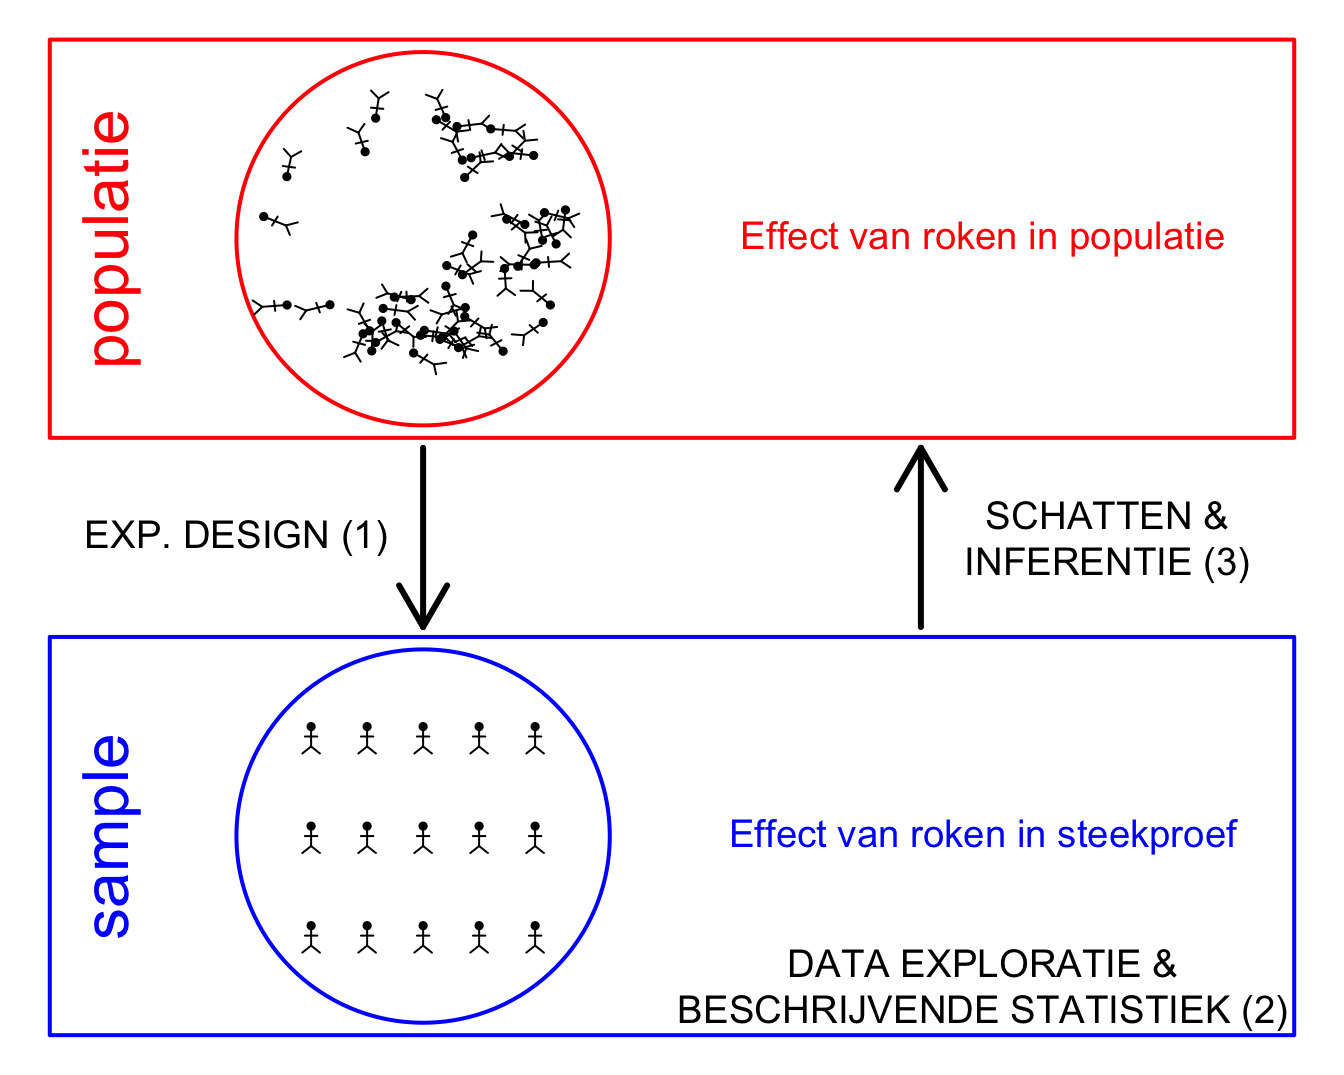
\includegraphics{experimentalDesignI_files/figure-latex/pop2Samp2Pop-1} \end{center}

\hypertarget{concepten}{%
\section{Concepten}\label{concepten}}

\begin{itemize}
\tightlist
\item
  Experimentele eenheden zijn representatief voor populatie:
  Randomisatie
\item
  Replicatie: technisch vs biologisch, steekproefgrootte - power
\item
  Bronnen van variabiliteit: technisch, biologisch, binnen en tussen
  subjecten.
\end{itemize}

\hypertarget{replicatie}{%
\section{Replicatie}\label{replicatie}}

Paper over replicatie in Nature Methods (2 pagina's)
{[}\href{https://www.nature.com/articles/nmeth.3091.pdf}{PDF}{]}

\hypertarget{voorbeeld}{%
\subsection{Voorbeeld}\label{voorbeeld}}

In een RNA-seq experiment willen de onderzoekers het effect nagaan van
een medicijn op de gen expressie.

Mogelijkse onderzoeksvraag

\begin{itemize}
\tightlist
\item
  Is er een verschil in gemiddelde gen expressie tussen behandelde en
  niet behandelde samples
\end{itemize}

\hypertarget{bronnen-van-variabiliteit}{%
\subsection{Bronnen van variabiliteit}\label{bronnen-van-variabiliteit}}

TABLE 1 NATURE METHODS \textbar{} VOL.11 NO.9 \textbar{} SEPTEMBER 2014
\textbar{} 879 - 880

\begin{longtable}[]{@{}
  >{\centering\arraybackslash}p{(\columnwidth - 4\tabcolsep) * \real{0.36}}
  >{\raggedright\arraybackslash}p{(\columnwidth - 4\tabcolsep) * \real{0.29}}
  >{\centering\arraybackslash}p{(\columnwidth - 4\tabcolsep) * \real{0.36}}@{}}
\toprule
& Replicate type & Replicate category\(^\text{a}\) \\
\midrule
\endhead
& Colonies & B \\
& Strains & B \\
Animal study subjects & Cohoused groups & B \\
& Gender & B \\
& Individuals & B \\
& & \\
& Organs from sacrificed animals & B \\
& Methods for dissociating cells from tissue & T \\
Sample preparation & Dissociation runs from given tissue sample & T \\
& Individual cells & B \\
& & \\
& RNA-seq library construction & T \\
& Runs from the library of a given cell & T \\
Sequencing & Reads from different transcript molecules &
V\(^\text{b}\) \\
& Reads with unique molecular identifier (UMI) from a given transcript
molecule & T \\
\bottomrule
\end{longtable}

\begin{enumerate}
\def\labelenumi{(\alph{enumi})}
\tightlist
\item
  Replicates are categorized as biological (B), technical (T) or of
  variable type (V).
\item
  Sequence reads serve diverse purposes depending on the application and
  how reads are used in analysis.
\end{enumerate}

\begin{center}\rule{0.5\linewidth}{0.5pt}\end{center}

\hypertarget{op-welk-niveau-moeten-we-repliceren}{%
\subsection{Op welk niveau moeten we
repliceren?}\label{op-welk-niveau-moeten-we-repliceren}}

\begin{itemize}
\tightlist
\item
  \(\text{var}(X)=\sigma^2_A+\sigma^2_C+\sigma^2_M=\sigma^2_{TOT}\)
\item
  \(\text{var}(\bar{X})=\frac{\sigma^2_A}{n_A}+\frac{\sigma^2_C}{n_A n_C} + \frac{\sigma^2_M}{n_A n_C n_M}\)
\end{itemize}

\includegraphics{https://media.springernature.com/full/springer-static/image/art\%3A10.1038\%2Fnmeth.3091/MediaObjects/41592_2014_Article_BFnmeth3091_Fig1_HTML.jpg}
Figure 1 NATURE METHODS \textbar{} VOL.11 NO.9 \textbar{} SEPTEMBER 2014
\textbar{} 879 - 880

\begin{enumerate}
\def\labelenumi{(\alph{enumi})}
\tightlist
\item
  Three levels of replication (two biological, one technical) with
  animal, cell and measurement replicates normally distributed with a
  mean across animals of 10 and ratio of variances 1:2:0.5. Solid green
  (biological) and blue (technical) dots show how a measurement of the
  expression (X = 12) samples from all three sources of variation.
  Distribution s.d. is shown as horizontal lines.
\item
  Expression variance, Var(X), and variance of expression mean,
  Var(\(\bar X\)), computed across 10,000 simulations of nAnCnM = 48
  measurements for unique combinations of the number of animals (nA = 1
  to 48), cells per animal (nC = 1 to 48) and technical replicate
  measurements per cell (nM = 1 and 3). The ratio of Var(X) and
  Var(\(\bar X\)) is the effective sample size, n, which corresponds to
  the equivalent number of statistically independent measurements.
  Horizontal dashed lines correspond to biological and total variation.
  Error bars on Var(X) show s.d. from the 10,000 simulated samples (nM =
  1).
\end{enumerate}

\begin{center}\rule{0.5\linewidth}{0.5pt}\end{center}

Waar ligt interesse?

\begin{itemize}
\item
  Karakteriseren van bronnen van variabiliteit in experiment
  ==\textgreater{} technische en biologische repeats zijn nodig
\item
  Voornamelijke interesse in schatten van effect van behandeling
  ==\textgreater{} focus op biologische repeats
\item
  Extra biologische repeats lumpen alle bronnen van variabiliteit:
  biologische + technische variabiliteit.
\item
  Goed experimenteel design vereist na denken over replicatie

  \begin{enumerate}
  \def\labelenumi{\arabic{enumi}.}
  \tightlist
  \item
    Identificeer onderzoeksvragen die men wenst te beantwoorden.
  \item
    Breng bronnen van variabiliteit in kaart in elke stap van het
    experiment
  \item
    Let op voor pseudoreplicatie, beoog zoveel mogelijk onafhankelijke
    repeats.
  \end{enumerate}
\end{itemize}

\begin{center}\rule{0.5\linewidth}{0.5pt}\end{center}

\hypertarget{power-steekproefgrootte-en-andere-design-aspecten.}{%
\section{Power, steekproefgrootte en andere design
aspecten.}\label{power-steekproefgrootte-en-andere-design-aspecten.}}

Reading materials:
\href{https://www.nature.com/articles/nmeth.2738.pdf}{Nature Methods
(2013), 10(12), 1139--1140}

\hypertarget{intermezzo-lineare-regression-in-matrix-vorm}{%
\subsection{Intermezzo lineare regression in matrix
vorm}\label{intermezzo-lineare-regression-in-matrix-vorm}}

\begin{itemize}
\tightlist
\item
  Lineaire regressie is een belangrijke methode in statistische data
  analyse.
\end{itemize}

\hypertarget{scalaire-vorm}{%
\subsubsection{Scalaire vorm}\label{scalaire-vorm}}

\begin{itemize}
\tightlist
\item
  Stel dat men voor elke experimentele eenheid \(p\) predictoren meet
  \(\mathbf{x}=(x_1,\ldots,x_p)\) en
\item
  continue respons \(Y\)
\item
  het linear regressiemodel kan dan worden geschreven als: \[
  Y=f(\mathbf{x}) +\epsilon=\beta_0+\sum\limits_{j=1}^p x_j\beta_j + \epsilon
  \] met i.i.d. \(\epsilon\sim N(0,\sigma^2)\)
\end{itemize}

\hypertarget{vectormatrix-vorm}{%
\subsubsection{Vector/Matrix vorm}\label{vectormatrix-vorm}}

\begin{itemize}
\tightlist
\item
  \(n\) observatie \((\mathbf{x}_1,y_1) \ldots (\mathbf{x}_n,y_n)\) with
  \(\mathbf{x}_1^T=[1 x_1 \ldots x_p]\)
\item
  Regressie in matrix notatie
  \[\mathbf{Y}=\mathbf{X\beta} + \mathbf{\epsilon}\] met
  \(\mathbf{Y}=\left[\begin{array}{c}y_1\\ \vdots\\y_n\end{array}\right]\),
  \(\mathbf{X}=\left[\begin{array}{cccc} 1&x_{11}&\ldots&x_{1p}\\ \vdots&\vdots&&\vdots\\ 1&x_{n1}&\ldots&x_{np} \end{array}\right]\)
  or
  \(\mathbf{X}=\left[\begin{array}{c} \mathbf{x}_1^T\\\vdots\\\mathbf{x}_n^T\end{array}\right]\),
  \(\boldsymbol{\beta}=\left[\begin{array}{c}\beta_0\\ \vdots\\ \beta_p\end{array}\right]\)
  and
  \(\mathbf{\epsilon}=\left[\begin{array}{c} \epsilon_1 \\ \vdots \\ \epsilon_n\end{array}\right]\)
\end{itemize}

\begin{center}\rule{0.5\linewidth}{0.5pt}\end{center}

\hypertarget{kleinste-kwadraten-techniekleast-squares-ls}{%
\subsection{kleinste kwadraten techniek/Least Squares
(LS)}\label{kleinste-kwadraten-techniekleast-squares-ls}}

\begin{itemize}
\item
  Minimimaliseer de residuele kwadratensom \begin{eqnarray*}
  RSS(\boldsymbol{\beta})&=&\sum\limits_{i=1}^n e^2_i\\
  &=&\sum\limits_{i=1}^n \left(y_i-\beta_0-\sum\limits_{j=1}^p x_{ij}\beta_j\right)^2
  \end{eqnarray*}
\item
  of in matrix notatie
\end{itemize}

\[
\text{RSS}(\boldsymbol{\beta})=(\mathbf{Y}-\mathbf{X\beta})^T(\mathbf{Y}-\mathbf{X\beta})
\]

\[\rightarrow \hat{\boldsymbol{\beta}}=\text{argmin}_\beta \text{ RSS}(\boldsymbol{\beta})\]

\begin{center}\rule{0.5\linewidth}{0.5pt}\end{center}

\hypertarget{minimimaliseer-rss}{%
\subsubsection{Minimimaliseer RSS}\label{minimimaliseer-rss}}

\[
\begin{array}{ccc}
\frac{\partial RSS}{\partial \boldsymbol{\beta}}&=&\mathbf{0}\\\\
\frac{(\mathbf{Y}-\mathbf{X\beta})^T(\mathbf{Y}-\mathbf{X}\boldsymbol{\beta})}{\partial \boldsymbol{\beta}}&=&\mathbf{0}\\\\
-2\mathbf{X}^T(\mathbf{Y}-\mathbf{X}\boldsymbol{\beta})&=&\mathbf{0}\\\\
\mathbf{X}^T\mathbf{X\beta}&=&\mathbf{X}^T\mathbf{Y}\\\\
\hat{\boldsymbol{\beta}}&=&(\mathbf{X}^T\mathbf{X})^{-1}\mathbf{X}^T\mathbf{Y}
\end{array}
\]

\begin{center}\rule{0.5\linewidth}{0.5pt}\end{center}

\hypertarget{variantie-schatter}{%
\subsection{Variantie schatter?}\label{variantie-schatter}}

\[
\begin{array}{ccl}
\hat{\boldsymbol{\Sigma}}_{\hat{\boldsymbol{\beta}}}
&=&\text{var}\left[(\mathbf{X}^T\mathbf{X})^{-1}\mathbf{X}^T\mathbf{Y}\right]\\\\
&=&(\mathbf{X}^T\mathbf{X})^{-1}\mathbf{X}^T\text{var}\left[\mathbf{Y}\right]\mathbf{X}(\mathbf{X}^T\mathbf{X})^{-1}\\\\
&=&(\mathbf{X}^T\mathbf{X})^{-1}\mathbf{X}^T(\mathbf{I}\sigma^2)\mathbf{X}(\mathbf{X}^T\mathbf{X})^{-1}
\\\\
&=&(\mathbf{X}^T\mathbf{X})^{-1}\mathbf{X}^T\mathbf{I}\quad\mathbf{X}(\mathbf{X}^T\mathbf{X})^{-1}\sigma^2\\\\
%\hat{\boldmath{\Sigma}}_{\hat{\boldsymbol{\beta}}}&=&(\mathbf{X}^T\mathbf{X})^{-1}\mathbf{X}^T \text{var}\left[\mathbf{Y}\right](\mathbf{X}^T\mathbf{X})^{-1}\mathbf{X}\\
&=&(\mathbf{X}^T\mathbf{X})^{-1}\mathbf{X}^T\mathbf{X}(\mathbf{X}^T\mathbf{X})^{-1}\sigma^2\\\\
&=&(\mathbf{X}^T\mathbf{X})^{-1}\sigma^2
\end{array}
\]

De onzekerheid op model parameters hangt dus af van de residuele
variabiliteit en het de proefopzet!

\begin{itemize}
\item
  Hoe groter \(\mathbf{X}^T\mathbf{X}\) hoe meer informatie het
  experiment zal hebben over de model parameters en hoe kleiner hun
  variantie en standaard errors!
\item
  Factoriële designs?
\item
  Designs with continue predictoren?
\end{itemize}

\begin{center}\rule{0.5\linewidth}{0.5pt}\end{center}

De effectgrootte van interesse is typisch een lineaire combinatie van de
model parameters,\\
\[
l_0 \times \beta_0 + l_1 \times \beta_1 + ... + l_{p-1} \times \beta_{p-1} = \mathbf{L}^T\boldsymbol{\beta}
\]

De nulhypothese van onze test kan dan worden geschreven als

\[
H_0: \mathbf{L}^T\boldsymbol{\beta} = 0 
\]

vs de alternatieve hypothese

\[
H_0: \mathbf{L}^T\boldsymbol{\beta} \neq 0 
\]

En het bewijs in het experiment tegen \(H_0\) kan worden gekwantificeerd
met de t-test statistiek:

\[
t=\frac{\mathbf{L}^T\hat{\boldsymbol{\beta}} - 0}{\text{se}_{\mathbf{L}^T\hat{\boldsymbol{\beta}}}}
\] die een t-distributie volgt met n-p vrijheidsgraden onder de nul
hypothese als alle aannames van het model geldig zijn.

De kracht van de toets is dan

\[P(p < 0.05 | H_1)\] en hangt af van

\begin{itemize}
\tightlist
\item
  de werkelijke effectgrootte in de populatie
  \(\mathbf{L}^T\boldsymbol{\beta}\).
\item
  Het aantal observaties: SE en df van t-test.
\item
  Keuze van de designpunten
\item
  Keuze van significantie-niveau \(\alpha\).
\end{itemize}

We kunnen dit evalueren aan de hand van simulaties.

\hypertarget{muis-voorbeeld}{%
\subsection{Muis voorbeeld}\label{muis-voorbeeld}}

\begin{itemize}
\item
  In 2021 publiceerden Choa et al.~dat cytokine Thymic stromal
  lymphopoietin (TSLP) vetverlies induceert bij muizen die een vet dieet
  krijgen door de secretie van talg.
  {[}\href{https://www.science.org/doi/full/10.1126/science.abd2893}{html}{]}
  {[}\href{https://www.science.org/doi/pdf/10.1126/science.abd2893}{PDF}{]}
\item
  Stel dat je een gelijkaardig experiment op wil zetten om na te gaan of
  cytokine interleukin 25 (IL) ook een effect heeft op het gewicht van
  muizen.
\item
  Je plant een studie met een controle groep muizen die een hoog vet
  dieet krijgen (HFD) en een behandelingsgroep die een HFD dieet met IL
  krijgt.
\item
  Wat is de vereiste steekproefgrootte om een bepaald effect op te
  pikken van de behandeling?
\end{itemize}

\hypertarget{hoe-zal-je-de-data-van-het-experiment-analyseren}{%
\subsubsection{Hoe zal je de data van het experiment
analyseren?}\label{hoe-zal-je-de-data-van-het-experiment-analyseren}}

\begin{center}\rule{0.5\linewidth}{0.5pt}\end{center}

\begin{itemize}
\item
  \(H_0\): Er is geen verschil in het gewicht van muizen die een dieet
  met IL krijgen en muizen die het controle dieet krijgen.
\item
  \(H_1\): Het gewicht is gemiddelde verschillend tussen muizen die het
  IL dieet krijgen en muizen die het controle dieet krijgen.
\item
  Two sample t-test of een t-test op de helling van het lineaire model
  met 1 dummy variabele
\end{itemize}

\[ Y_i = \beta_0 + \beta_1 X_\text{iIL} + \epsilon_i\]

\[
\text{met }
X_\text{iIL}=\begin{cases}X_{iIL}=0 & \text{HFD}\\X_{iIL}=1 & \text{HFD + IL}\end{cases}.
\]

\begin{itemize}
\tightlist
\item
  Geschatte effectgrootte?
\end{itemize}

\[\hat\delta = \bar X_{IL} - \bar X_{c} = \hat \beta_1\]

\begin{itemize}
\tightlist
\item
  Test statistiek \[
  T = \frac{\bar{X}_{IL}-\bar{X}_{c}}{SD_\text{pooled} \times \sqrt{\frac{1}{n_1} + \frac{1}{n_2}}} = \frac{\hat\beta_1}{\text{SE}_{\hat\beta_1}}
  \]
\item
  \(\hat \beta_1\) is een onvertekende schatter van het werkelijk
  gewichtsverschil (\(\delta =\mu_{IL}-\mu_{c} = \beta_1\)) dat zou
  voorkomen in de populatie van muizen gevoed met HFD vs muizen gevoed
  met HFD + IL.
\end{itemize}

\hypertarget{power}{%
\subsubsection{Power?}\label{power}}

\[
P[p < \alpha \vert \beta_1 \neq 0]
\]

De kracht (power) zal dus afhangen van

\begin{itemize}
\tightlist
\item
  Het werkelijke gemiddelde gewichtsverschil \(\beta_1\) in de
  populatie.
\item
  De variabiliteit van de gewichtsmetingen
\item
  het significantie-niveau \(\alpha\)
\item
  steekproefgrootte \(n_{IL}\) en \(n_c\) in beide groepen
\end{itemize}

We kunnen de power schatten als

\begin{enumerate}
\def\labelenumi{\arabic{enumi}.}
\tightlist
\item
  voldaan is aan de aannamens van het model: gewicht in beide groepen is
  normaal verdeeld met gelijke variantie
\end{enumerate}

en als we de

\begin{enumerate}
\def\labelenumi{\arabic{enumi}.}
\setcounter{enumi}{1}
\item
  standaard deviatie kennen van gewichtsmetingen rond hun
  groepsgemiddelde voor muizen die een HFD diet krijgen
\item
  de echte effectgrootte in de populatie
\item
  \(n_1\) en \(n_2\)
\end{enumerate}

\hypertarget{gebruik-data-uit-vorig-experiment-om-inzicht-te-krijgen-in-de-gewichtsdata-van-muizen}{%
\subsubsection{Gebruik data uit vorig experiment om inzicht te krijgen
in de gewichtsdata van
muizen}\label{gebruik-data-uit-vorig-experiment-om-inzicht-te-krijgen-in-de-gewichtsdata-van-muizen}}

Stel dat we toegang hebben tot data van een vorig experiment (hier dat
van Karen Svenson en Dan Gatti, gefinancierd door P50 GM070683 en
beschikbaar op
\href{http://genomicsclass.github.io/book/pages/random_variables.html}{PH525x})

\begin{Shaded}
\begin{Highlighting}[]
\NormalTok{mice }\OtherTok{\textless{}{-}} \FunctionTok{read.csv}\NormalTok{(}\StringTok{"https://raw.githubusercontent.com/genomicsclass/dagdata/master/inst/extdata/femaleMiceWeights.csv"}\NormalTok{)}

\NormalTok{mice }\SpecialCharTok{\%\textgreater{}\%} 
  \FunctionTok{ggplot}\NormalTok{(}\FunctionTok{aes}\NormalTok{(}\AttributeTok{x=}\NormalTok{Diet,}\AttributeTok{y=}\NormalTok{Bodyweight)) }\SpecialCharTok{+}
  \FunctionTok{geom\_boxplot}\NormalTok{(}\AttributeTok{outlier.shape=}\ConstantTok{FALSE}\NormalTok{) }\SpecialCharTok{+}
  \FunctionTok{geom\_jitter}\NormalTok{()}
\end{Highlighting}
\end{Shaded}

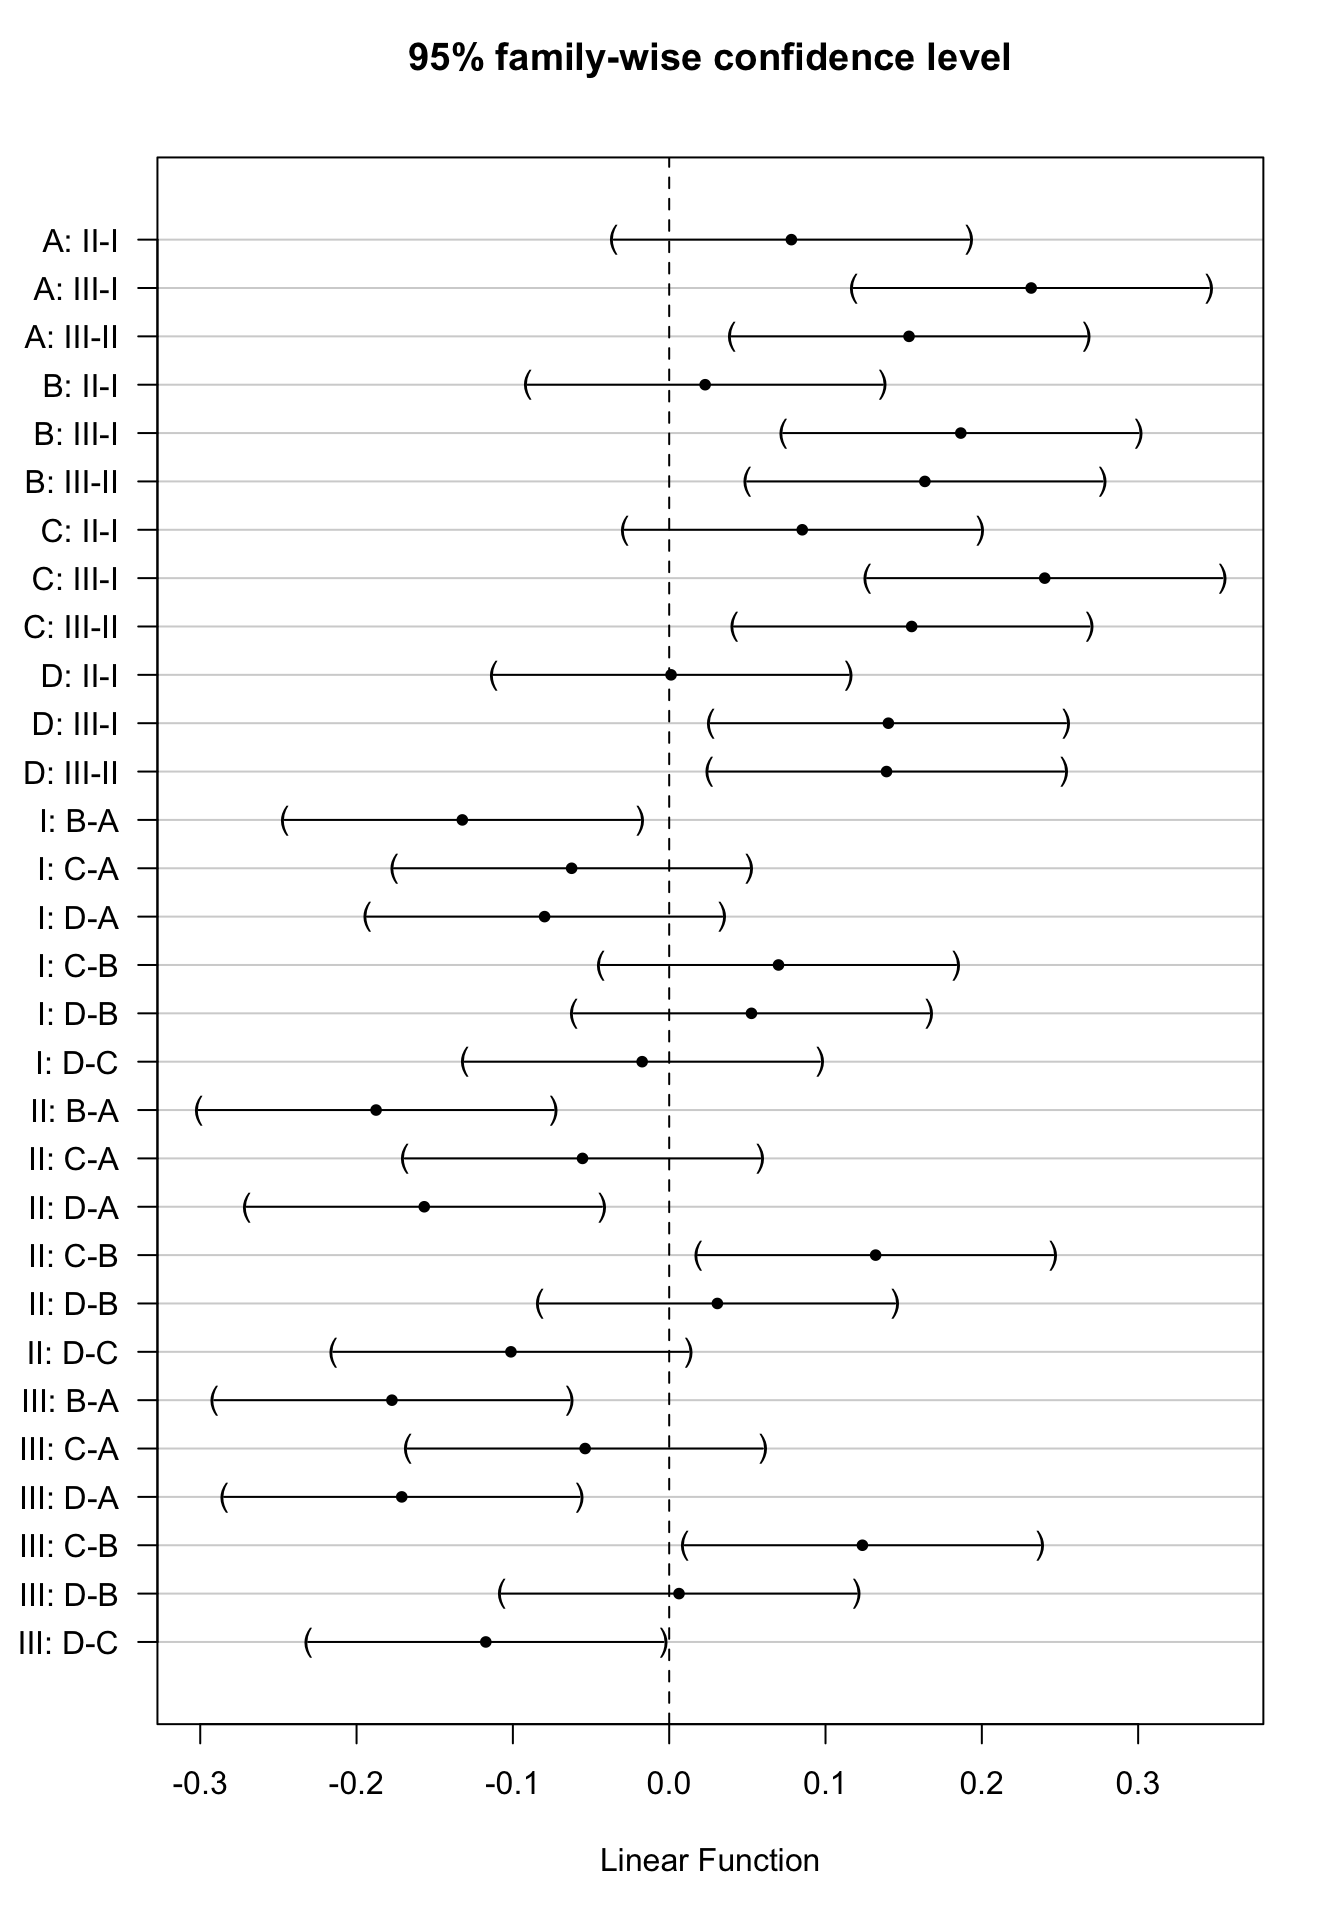
\includegraphics{experimentalDesignI_files/figure-latex/unnamed-chunk-11-1.pdf}

\begin{Shaded}
\begin{Highlighting}[]
\NormalTok{mice }\SpecialCharTok{\%\textgreater{}\%} 
  \FunctionTok{ggplot}\NormalTok{(}\FunctionTok{aes}\NormalTok{(}\AttributeTok{sample=}\NormalTok{Bodyweight)) }\SpecialCharTok{+}
  \FunctionTok{geom\_qq}\NormalTok{() }\SpecialCharTok{+} 
  \FunctionTok{geom\_qq\_line}\NormalTok{() }\SpecialCharTok{+}
  \FunctionTok{facet\_wrap}\NormalTok{(}\SpecialCharTok{\textasciitilde{}}\NormalTok{Diet)}
\end{Highlighting}
\end{Shaded}

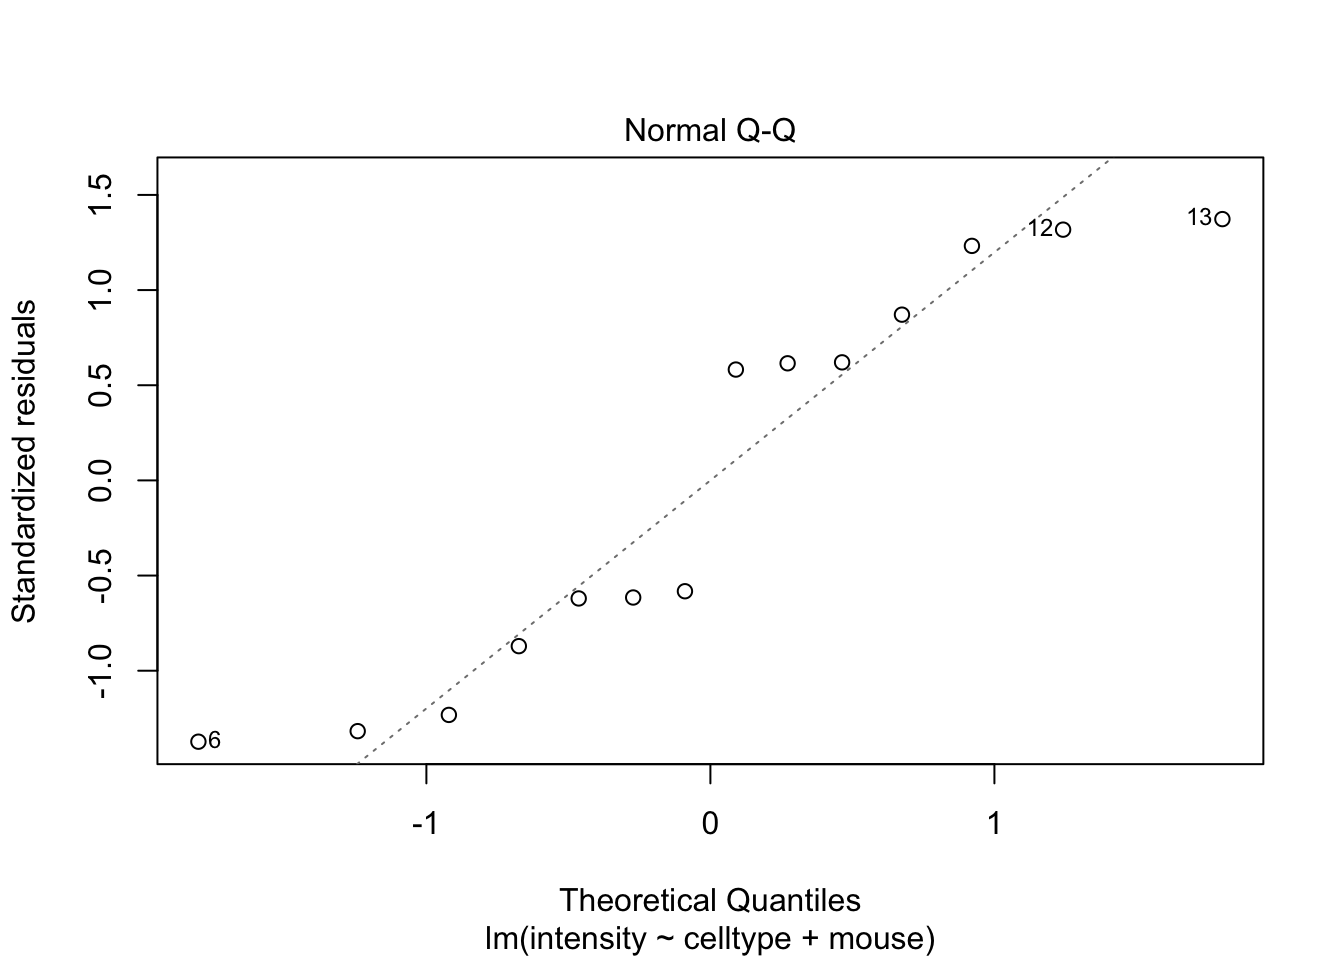
\includegraphics{experimentalDesignI_files/figure-latex/unnamed-chunk-11-2.pdf}

\begin{Shaded}
\begin{Highlighting}[]
\NormalTok{mice }\OtherTok{\textless{}{-}}\NormalTok{ mice }\SpecialCharTok{\%\textgreater{}\%} \FunctionTok{mutate}\NormalTok{(}\AttributeTok{Diet =} \FunctionTok{as.factor}\NormalTok{(Diet))}
\NormalTok{miceSum }\OtherTok{\textless{}{-}}\NormalTok{ mice }\SpecialCharTok{\%\textgreater{}\%} 
  \FunctionTok{group\_by}\NormalTok{(Diet)  }\SpecialCharTok{\%\textgreater{}\%}
  \FunctionTok{summarize\_at}\NormalTok{(}\StringTok{"Bodyweight"}\NormalTok{,}\FunctionTok{list}\NormalTok{(}\AttributeTok{mean=}\SpecialCharTok{\textasciitilde{}}\FunctionTok{mean}\NormalTok{(.,}\AttributeTok{na.rm=}\ConstantTok{TRUE}\NormalTok{),}
                    \AttributeTok{sd=}\SpecialCharTok{\textasciitilde{}}\FunctionTok{sd}\NormalTok{(.,}\AttributeTok{na.rm=}\ConstantTok{TRUE}\NormalTok{),}
                    \AttributeTok{n=}\ControlFlowTok{function}\NormalTok{(x) x}\SpecialCharTok{\%\textgreater{}\%}\NormalTok{is.na}\SpecialCharTok{\%\textgreater{}\%}\StringTok{\textasciigrave{}}\AttributeTok{!}\StringTok{\textasciigrave{}}\SpecialCharTok{\%\textgreater{}\%}\NormalTok{sum)) }\SpecialCharTok{\%\textgreater{}\%}
  \FunctionTok{mutate}\NormalTok{(}\AttributeTok{se=}\NormalTok{sd}\SpecialCharTok{/}\FunctionTok{sqrt}\NormalTok{(n))}
\NormalTok{miceSum }
\end{Highlighting}
\end{Shaded}

\begin{verbatim}
# A tibble: 2 x 5
  Diet   mean    sd     n    se
  <fct> <dbl> <dbl> <int> <dbl>
1 chow   23.8  3.02    12 0.873
2 hf     26.8  4.10    12 1.18 
\end{verbatim}

In het experiment werden twee diëten gebruikt:

\begin{itemize}
\tightlist
\item
  gewoon diet o.b.v. granen (Chow)
\item
  Heel vet dieet (high fat: hf)
\end{itemize}

We kunnen de data van de hf muizen gebruiken als input voor onze power
analyse.

\begin{itemize}
\tightlist
\item
  De data van hf muizen lijken normaal verdeeld te zijn.\\
\item
  Het gemiddelde gewicht van een hf muis is 26.8g
\item
  De standaard deviatie (SD) van het gewicht van hf muizen is 4.1g
\end{itemize}

Effectgroote?

\begin{itemize}
\tightlist
\item
  De alternative hypothese is complex.
\item
  Omvat alle mogelijke effecten!
\item
  Om een power analyse te doen kiezen we daarom een minimale
  effectgrootte die we wensen op te pikken in het nieuwe experiment.
\item
  Veronderstel dat we een gewichtsverschil willen oppikken van minimaal
  10\%.
\end{itemize}

\begin{Shaded}
\begin{Highlighting}[]
\NormalTok{delta }\OtherTok{\textless{}{-}} \SpecialCharTok{{-}} \FunctionTok{round}\NormalTok{(miceSum}\SpecialCharTok{$}\NormalTok{mean[}\DecValTok{2}\NormalTok{] }\SpecialCharTok{*}\NormalTok{.}\DecValTok{1}\NormalTok{,}\DecValTok{1}\NormalTok{)}
\NormalTok{delta}
\end{Highlighting}
\end{Shaded}

\begin{verbatim}
[1] -2.7
\end{verbatim}

Merk op dat het gemiddeld gewicht dan dicht komt bij dat van muizen in
het pilootexperiment die werden gevoed met het normale dieet.

We kunnen nu een simulatie studie opzetten om de power te berekenen voor
een experiment met 8 muizen in elke groep.

\hypertarget{euxe9n-simulatie}{%
\paragraph{Eén simulatie}\label{euxe9n-simulatie}}

\begin{Shaded}
\begin{Highlighting}[]
\FunctionTok{set.seed}\NormalTok{(}\DecValTok{1423}\NormalTok{)}
\NormalTok{n1 }\OtherTok{\textless{}{-}}\NormalTok{ n2 }\OtherTok{\textless{}{-}} \DecValTok{8}
\NormalTok{b0 }\OtherTok{\textless{}{-}} \FunctionTok{round}\NormalTok{(miceSum}\SpecialCharTok{$}\NormalTok{mean[}\DecValTok{2}\NormalTok{],}\DecValTok{1}\NormalTok{)}
\NormalTok{b1 }\OtherTok{\textless{}{-}} \SpecialCharTok{{-}}\NormalTok{ delta}
\NormalTok{sd }\OtherTok{\textless{}{-}} \FunctionTok{round}\NormalTok{(miceSum}\SpecialCharTok{$}\NormalTok{sd[}\DecValTok{2}\NormalTok{],}\DecValTok{1}\NormalTok{)}
\NormalTok{alpha }\OtherTok{\textless{}{-}} \FloatTok{0.05}

\NormalTok{x }\OtherTok{\textless{}{-}} \FunctionTok{rep}\NormalTok{(}\DecValTok{0}\SpecialCharTok{:}\DecValTok{1}\NormalTok{,}\FunctionTok{c}\NormalTok{(n1,n2))}
\NormalTok{y }\OtherTok{\textless{}{-}}\NormalTok{ b0 }\SpecialCharTok{+}\NormalTok{ b1 }\SpecialCharTok{*}\NormalTok{ x }\SpecialCharTok{+} \FunctionTok{rnorm}\NormalTok{(n1}\SpecialCharTok{+}\NormalTok{n2,}\DecValTok{0}\NormalTok{, }\AttributeTok{sd =}\NormalTok{ sd)}
\NormalTok{fit }\OtherTok{\textless{}{-}} \FunctionTok{lm}\NormalTok{(y}\SpecialCharTok{\textasciitilde{}}\NormalTok{x)}
\NormalTok{bhat }\OtherTok{\textless{}{-}}\NormalTok{ fit}\SpecialCharTok{$}\NormalTok{coef }
\NormalTok{stat }\OtherTok{\textless{}{-}} \FunctionTok{summary}\NormalTok{(fit)}
\FunctionTok{summary}\NormalTok{(fit)}\SpecialCharTok{$}\NormalTok{coef[}\DecValTok{2}\NormalTok{,]}
\end{Highlighting}
\end{Shaded}

\begin{verbatim}
  Estimate Std. Error    t value   Pr(>|t|) 
 2.5972480  1.7919658  1.4493848  0.1692595 
\end{verbatim}

Voor het gesimuleerde experiment konden we het effect van de behandeling
niet oppikken bij het \(\alpha\)=0.05 (p = 0.17) significantie-niveau!

\begin{itemize}
\tightlist
\item
  We moeten het experiment herhalen om de power te schatten.
\item
  We zullen de simulatie daarom coderen in een functie die we kunnen
  hergebruiken.
\end{itemize}

\hypertarget{simulatie-van-herhaalde-experimenten-repeated-experiments}{%
\paragraph{Simulatie van herhaalde experimenten (repeated
experiments)}\label{simulatie-van-herhaalde-experimenten-repeated-experiments}}

\begin{Shaded}
\begin{Highlighting}[]
\FunctionTok{library}\NormalTok{(multcomp)}
\NormalTok{n1 }\OtherTok{\textless{}{-}}\NormalTok{ n2 }\OtherTok{\textless{}{-}} \DecValTok{8}

\NormalTok{b0 }\OtherTok{\textless{}{-}} \FunctionTok{round}\NormalTok{(miceSum}\SpecialCharTok{$}\NormalTok{mean[}\DecValTok{2}\NormalTok{],}\DecValTok{1}\NormalTok{)}
\NormalTok{b1 }\OtherTok{\textless{}{-}} \SpecialCharTok{{-}}\NormalTok{ delta}

\NormalTok{sd }\OtherTok{\textless{}{-}} \FunctionTok{round}\NormalTok{(miceSum}\SpecialCharTok{$}\NormalTok{sd[}\DecValTok{2}\NormalTok{],}\DecValTok{1}\NormalTok{)}
\NormalTok{predictorData }\OtherTok{\textless{}{-}} \FunctionTok{data.frame}\NormalTok{(}\AttributeTok{Diet =} \FunctionTok{rep}\NormalTok{(}\FunctionTok{c}\NormalTok{(}\StringTok{"c"}\NormalTok{,}\StringTok{"hf"}\NormalTok{),}\FunctionTok{c}\NormalTok{(n1,n2)) }\SpecialCharTok{\%\textgreater{}\%}\NormalTok{ as.factor)}

\NormalTok{alpha }\OtherTok{\textless{}{-}} \FloatTok{0.05}

\NormalTok{simLm }\OtherTok{\textless{}{-}} \ControlFlowTok{function}\NormalTok{(form, data, betas, sd, contrasts, }\AttributeTok{simIndex =} \ConstantTok{NA}\NormalTok{)}
\NormalTok{\{}
\NormalTok{  dataSim }\OtherTok{\textless{}{-}}\NormalTok{ data}
\NormalTok{  X }\OtherTok{\textless{}{-}} \FunctionTok{model.matrix}\NormalTok{(form,dataSim)}
\NormalTok{  dataSim}\SpecialCharTok{$}\NormalTok{ySim }\OtherTok{\textless{}{-}}\NormalTok{ X}\SpecialCharTok{\%*\%}\NormalTok{betas }\SpecialCharTok{+} \FunctionTok{rnorm}\NormalTok{(}\FunctionTok{nrow}\NormalTok{(dataSim),}\DecValTok{0}\NormalTok{,sd)}
\NormalTok{  form }\OtherTok{\textless{}{-}} \FunctionTok{formula}\NormalTok{(}\FunctionTok{paste}\NormalTok{(}\StringTok{"ySim \textasciitilde{}"}\NormalTok{,form[[}\DecValTok{2}\NormalTok{]]))}
\NormalTok{  fitSim }\OtherTok{\textless{}{-}} \FunctionTok{lm}\NormalTok{(form,dataSim)}
\NormalTok{  mcp }\OtherTok{\textless{}{-}} \FunctionTok{glht}\NormalTok{(fitSim,}\AttributeTok{linfct =}\NormalTok{ contrasts)}
  \FunctionTok{return}\NormalTok{(}\FunctionTok{summary}\NormalTok{(mcp)}\SpecialCharTok{$}\NormalTok{test[}\FunctionTok{c}\NormalTok{(}\StringTok{"coefficients"}\NormalTok{,}\StringTok{"sigma"}\NormalTok{,}\StringTok{"tstat"}\NormalTok{,}\StringTok{"pvalues"}\NormalTok{)]}\SpecialCharTok{\%\textgreater{}\%}\NormalTok{ unlist)}
\NormalTok{\}}

\FunctionTok{simLm}\NormalTok{(}
  \AttributeTok{form =} \SpecialCharTok{\textasciitilde{}}\NormalTok{Diet,}
  \AttributeTok{data =}\NormalTok{ predictorData,}
  \AttributeTok{betas =} \FunctionTok{c}\NormalTok{(b0,b1),}
  \AttributeTok{sd =}\NormalTok{ sd,}
  \AttributeTok{contrasts =} \StringTok{"Diethf = 0"}\NormalTok{)}
\end{Highlighting}
\end{Shaded}

\begin{verbatim}
coefficients.Diethf        sigma.Diethf        tstat.Diethf             pvalues 
          1.9444623           2.0931302           0.9289734           0.3686439 
\end{verbatim}

We hebben nu een generiek functie waarmee we data kunnen simuleren die
normaal verdeeld zijn voor elk mogelijk design die we met het lineair
model kunnen analyseren.

De functie heeft volgende argumenten:

\begin{itemize}
\tightlist
\item
  \texttt{form}: One sided formula including the structure of the
  predictors in the model
\item
  \texttt{data}: Data frame with the predictor values for the design
\item
  \texttt{betas}: A vector with values for all mean model parameters
\item
  \texttt{sd}: The standard deviation of the error
\item
  \texttt{contrasts}: a scalar or a vector with the null hypotheses that
  we would like to assess.
\item
  \texttt{simIndex}: an arbitrary argument that is not used by the
  function but that will allow it to be used in an sapply loop that runs
  from 1 up to the number of simulations.
\end{itemize}

Simuleer nSim = 1000 herhaalde experimenten:

\begin{Shaded}
\begin{Highlighting}[]
\FunctionTok{set.seed}\NormalTok{(}\DecValTok{1425}\NormalTok{)}
\NormalTok{nSim }\OtherTok{\textless{}{-}} \DecValTok{1000}

\NormalTok{simResults  }\OtherTok{\textless{}{-}} \FunctionTok{t}\NormalTok{(}\FunctionTok{sapply}\NormalTok{(}\DecValTok{1}\SpecialCharTok{:}\NormalTok{nSim,simLm,}\AttributeTok{form =} \SpecialCharTok{\textasciitilde{}}\NormalTok{Diet,}\AttributeTok{data =}\NormalTok{ predictorData,}\AttributeTok{betas =} \FunctionTok{c}\NormalTok{(b0,b1),}\AttributeTok{sd =}\NormalTok{ sd,}\AttributeTok{contrasts =} \StringTok{"Diethf = 0"}\NormalTok{))}
\NormalTok{power }\OtherTok{\textless{}{-}} \FunctionTok{mean}\NormalTok{(simResults[,}\DecValTok{4}\NormalTok{] }\SpecialCharTok{\textless{}}\NormalTok{ alpha)}
\NormalTok{power}
\end{Highlighting}
\end{Shaded}

\begin{verbatim}
[1] 0.221
\end{verbatim}

We hebben een power van 22.1\% om het behandelingseffect op te pikken
met 8 biologische herhalingen in elke behandelingsgroep.

Merk op dat de power van een experiment ook het hoogste is als het
aantal observaties gebalanceerd is, m.a.w. \(n_1=n_2\).

\hypertarget{power-voor-verschillende-steekproefgroottes}{%
\paragraph{Power voor verschillende
steekproefgroottes}\label{power-voor-verschillende-steekproefgroottes}}

We kunnen de power nu berekenen voor meerdere steekproefgrootes.

\begin{Shaded}
\begin{Highlighting}[]
\NormalTok{power }\OtherTok{\textless{}{-}} \FunctionTok{data.frame}\NormalTok{(}\AttributeTok{n=}\FunctionTok{c}\NormalTok{(}\DecValTok{3}\NormalTok{,}\DecValTok{5}\NormalTok{,}\DecValTok{10}\NormalTok{,}\DecValTok{25}\NormalTok{,}\DecValTok{50}\NormalTok{,}\DecValTok{75}\NormalTok{,}\DecValTok{100}\NormalTok{),}\AttributeTok{power=}\ConstantTok{NA}\NormalTok{)}

\ControlFlowTok{for}\NormalTok{ (i }\ControlFlowTok{in} \DecValTok{1}\SpecialCharTok{:}\FunctionTok{nrow}\NormalTok{(power))}
\NormalTok{\{}
\NormalTok{  n1 }\OtherTok{\textless{}{-}}\NormalTok{ n2 }\OtherTok{\textless{}{-}}\NormalTok{ power}\SpecialCharTok{$}\NormalTok{n[i]}
\NormalTok{  predictorData }\OtherTok{\textless{}{-}} \FunctionTok{data.frame}\NormalTok{(}\AttributeTok{Diet =} \FunctionTok{rep}\NormalTok{(}\FunctionTok{c}\NormalTok{(}\StringTok{"c"}\NormalTok{,}\StringTok{"hf"}\NormalTok{),}\FunctionTok{c}\NormalTok{(n1,n2)) }\SpecialCharTok{\%\textgreater{}\%}\NormalTok{ as.factor)}
\NormalTok{  simResults  }\OtherTok{\textless{}{-}} \FunctionTok{t}\NormalTok{(}\FunctionTok{sapply}\NormalTok{(}\DecValTok{1}\SpecialCharTok{:}\NormalTok{nSim,simLm,}\AttributeTok{form =} \SpecialCharTok{\textasciitilde{}}\NormalTok{Diet,}\AttributeTok{data =}\NormalTok{ predictorData,}\AttributeTok{betas =} \FunctionTok{c}\NormalTok{(b0,b1),}\AttributeTok{sd =}\NormalTok{ sd,}\AttributeTok{contrasts =} \StringTok{"Diethf = 0"}\NormalTok{))}
\NormalTok{  power}\SpecialCharTok{$}\NormalTok{power[i] }\OtherTok{\textless{}{-}} \FunctionTok{mean}\NormalTok{(simResults[,}\StringTok{"pvalues"}\NormalTok{] }\SpecialCharTok{\textless{}}\NormalTok{ alpha)}
\NormalTok{\}}
\NormalTok{power}
\end{Highlighting}
\end{Shaded}

\begin{verbatim}
    n power
1   3 0.114
2   5 0.158
3  10 0.304
4  25 0.648
5  50 0.890
6  75 0.982
7 100 0.998
\end{verbatim}

\begin{Shaded}
\begin{Highlighting}[]
\NormalTok{power }\SpecialCharTok{\%\textgreater{}\%} 
  \FunctionTok{ggplot}\NormalTok{(}\FunctionTok{aes}\NormalTok{(}\AttributeTok{x=}\NormalTok{n,}\AttributeTok{y=}\NormalTok{power)) }\SpecialCharTok{+}
  \FunctionTok{geom\_line}\NormalTok{()}
\end{Highlighting}
\end{Shaded}

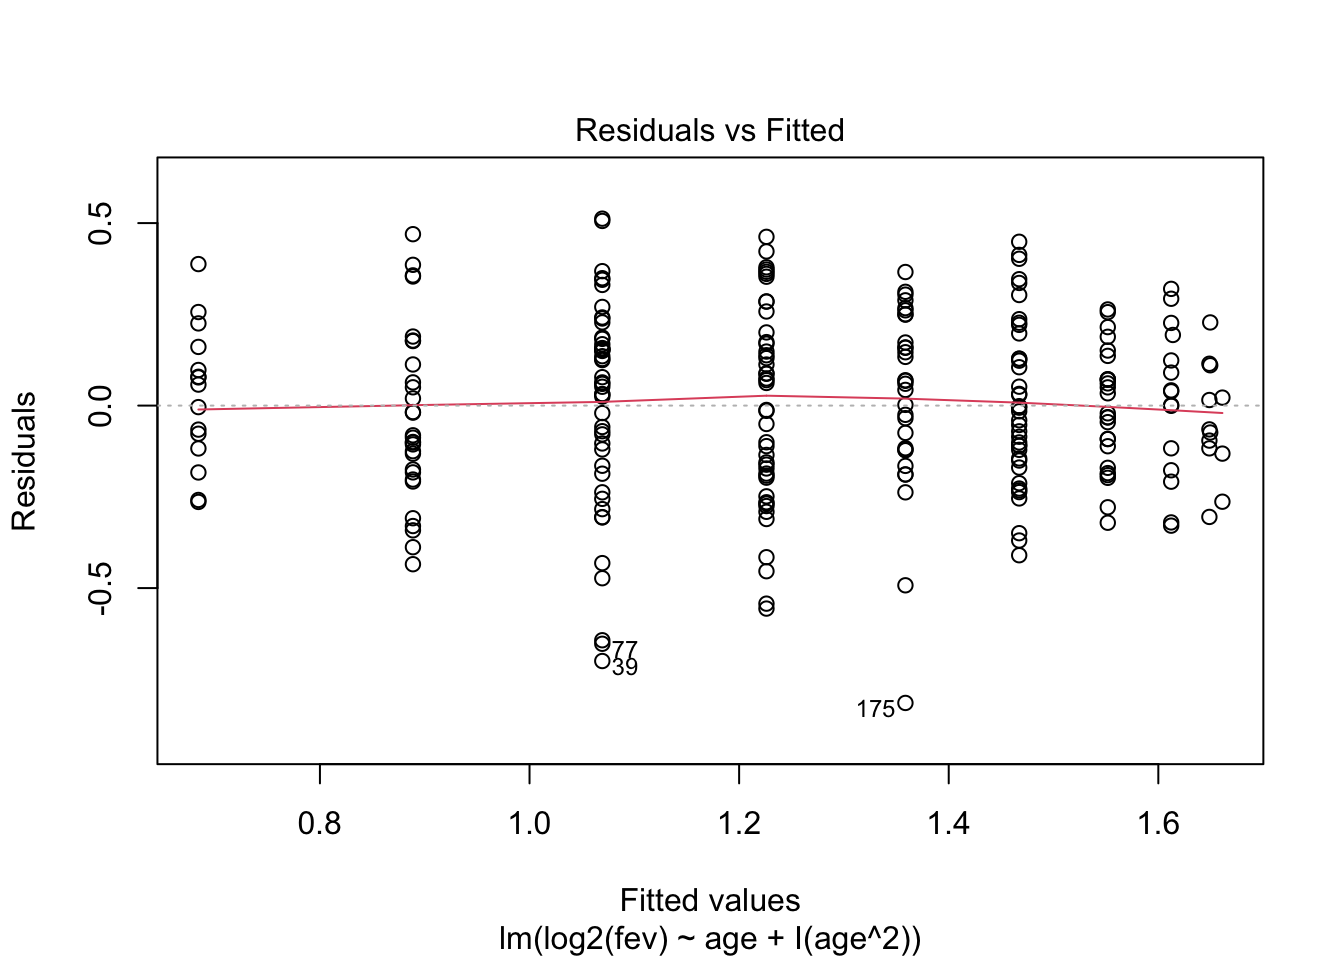
\includegraphics{experimentalDesignI_files/figure-latex/unnamed-chunk-18-1.pdf}

\hypertarget{bestudeer-power-in-functie-van-steekproefgrootte-en-effectgrootte}{%
\paragraph{Bestudeer power in functie van steekproefgrootte en
effectgrootte}\label{bestudeer-power-in-functie-van-steekproefgrootte-en-effectgrootte}}

Merk op dat

\begin{itemize}
\tightlist
\item
  het teken van delta arbitrair is omdat we tweezijdig testen.
\item
  het intercept arbitrair is omdat we alleen testen op \(\beta_1\)
\item
  We nemen daarom typisch \(\beta_0 = 0\)
\end{itemize}

\begin{Shaded}
\begin{Highlighting}[]
\NormalTok{nSim }\OtherTok{\textless{}{-}} \DecValTok{1000}
\NormalTok{b0 }\OtherTok{\textless{}{-}} \DecValTok{0}
\NormalTok{deltas }\OtherTok{\textless{}{-}} \FunctionTok{c}\NormalTok{(}\DecValTok{1}\NormalTok{,}\DecValTok{2}\NormalTok{,}\DecValTok{3}\NormalTok{,}\DecValTok{5}\NormalTok{,}\DecValTok{10}\NormalTok{)}
\NormalTok{sd }\OtherTok{\textless{}{-}} \FunctionTok{round}\NormalTok{(miceSum}\SpecialCharTok{$}\NormalTok{sd[}\DecValTok{2}\NormalTok{],}\DecValTok{1}\NormalTok{)}
\NormalTok{ns }\OtherTok{\textless{}{-}}  \FunctionTok{c}\NormalTok{(}\DecValTok{3}\NormalTok{,}\DecValTok{5}\NormalTok{,}\DecValTok{10}\NormalTok{,}\DecValTok{20}\NormalTok{,}\DecValTok{25}\NormalTok{,}\DecValTok{50}\NormalTok{,}\DecValTok{75}\NormalTok{,}\DecValTok{100}\NormalTok{)  }

\NormalTok{power }\OtherTok{\textless{}{-}} \FunctionTok{data.frame}\NormalTok{(}\AttributeTok{b1=}\FunctionTok{rep}\NormalTok{(deltas,}\AttributeTok{each=}\FunctionTok{length}\NormalTok{(ns)),}
                    \AttributeTok{n=}\FunctionTok{rep}\NormalTok{(ns,}\FunctionTok{length}\NormalTok{(deltas)),}
                    \AttributeTok{power=}\ConstantTok{NA}\NormalTok{)}

\ControlFlowTok{for}\NormalTok{ (i }\ControlFlowTok{in} \DecValTok{1}\SpecialCharTok{:}\FunctionTok{nrow}\NormalTok{(power))}
\NormalTok{\{}
\NormalTok{  b1 }\OtherTok{\textless{}{-}}\NormalTok{power}\SpecialCharTok{$}\NormalTok{b1[i]}
\NormalTok{  n1 }\OtherTok{\textless{}{-}}\NormalTok{ n2 }\OtherTok{\textless{}{-}}\NormalTok{  power}\SpecialCharTok{$}\NormalTok{n[i]}
\NormalTok{  predictorData }\OtherTok{\textless{}{-}} \FunctionTok{data.frame}\NormalTok{(}\AttributeTok{Diet =} \FunctionTok{rep}\NormalTok{(}\FunctionTok{c}\NormalTok{(}\StringTok{"c"}\NormalTok{,}\StringTok{"hf"}\NormalTok{),}\FunctionTok{c}\NormalTok{(n1,n2)) }\SpecialCharTok{\%\textgreater{}\%}\NormalTok{ as.factor)}
\NormalTok{  simResults  }\OtherTok{\textless{}{-}} \FunctionTok{t}\NormalTok{(}\FunctionTok{sapply}\NormalTok{(}\DecValTok{1}\SpecialCharTok{:}\NormalTok{nSim,simLm,}\AttributeTok{form =} \SpecialCharTok{\textasciitilde{}}\NormalTok{Diet,}\AttributeTok{data =}\NormalTok{ predictorData,}\AttributeTok{betas =} \FunctionTok{c}\NormalTok{(b0,b1),}\AttributeTok{sd =}\NormalTok{ sd,}\AttributeTok{contrasts =} \StringTok{"Diethf = 0"}\NormalTok{))}
\NormalTok{  power}\SpecialCharTok{$}\NormalTok{power[i] }\OtherTok{\textless{}{-}} \FunctionTok{mean}\NormalTok{(simResults[,}\StringTok{"pvalues"}\NormalTok{] }\SpecialCharTok{\textless{}}\NormalTok{ alpha)}
\NormalTok{\}}
\end{Highlighting}
\end{Shaded}

\begin{Shaded}
\begin{Highlighting}[]
\NormalTok{power }\SpecialCharTok{\%\textgreater{}\%} 
  \FunctionTok{ggplot}\NormalTok{(}\FunctionTok{aes}\NormalTok{(}\AttributeTok{x=}\NormalTok{n,}\AttributeTok{y=}\NormalTok{power,}\AttributeTok{col=}\NormalTok{b1}\SpecialCharTok{\%\textgreater{}\%}\NormalTok{as.factor)) }\SpecialCharTok{+}
  \FunctionTok{geom\_line}\NormalTok{()}
\end{Highlighting}
\end{Shaded}

\includegraphics{experimentalDesignI_files/figure-latex/unnamed-chunk-20-1.pdf}

Merk op dat de power curves wat schokkerig zijn omdat we maar een
beperkt aantal steekproefgroottes en een beperkt aantal simulaties
uitvoerden. Voor de lage powers is het aantal simulaties zeker
onvoldoende om heel betrouwbare schattingen van de power te bekomen.

\hypertarget{opmerkingen}{%
\section{Opmerkingen}\label{opmerkingen}}

\begin{itemize}
\item
  De code kan eenvoudig aangepast worden naar andere designs (zie
  oefeningen)

  \begin{itemize}
  \tightlist
  \item
    predictor data
  \item
    formula
  \item
    contrast
  \end{itemize}
\item
  De simulaties kunnen lang duren wanneer je veel scenario's evalueert.

  \begin{itemize}
  \tightlist
  \item
    Meer efficiënte code met matrices
  \item
    Voor two group comparison bestaat een analytische oplossing.
  \end{itemize}
\end{itemize}

\hypertarget{meer-efficiuxebnte-code-met-matrices}{%
\subsection{Meer efficiënte code met
matrices}\label{meer-efficiuxebnte-code-met-matrices}}

Code is veel sneller. We simulaleren nu 20 keer meer experimenten in een
veel kortere tijd!

\begin{Shaded}
\begin{Highlighting}[]
\NormalTok{nSim }\OtherTok{\textless{}{-}} \DecValTok{20000}
\NormalTok{b0 }\OtherTok{\textless{}{-}} \DecValTok{0}
\NormalTok{sd }\OtherTok{\textless{}{-}} \FunctionTok{round}\NormalTok{(miceSum}\SpecialCharTok{$}\NormalTok{sd[}\DecValTok{2}\NormalTok{],}\DecValTok{1}\NormalTok{)}
\NormalTok{ns }\OtherTok{\textless{}{-}}  \FunctionTok{c}\NormalTok{(}\DecValTok{3}\NormalTok{,}\DecValTok{5}\NormalTok{,}\DecValTok{10}\NormalTok{,}\DecValTok{20}\NormalTok{,}\DecValTok{25}\NormalTok{,}\DecValTok{50}\NormalTok{,}\DecValTok{75}\NormalTok{,}\DecValTok{100}\NormalTok{)  }
\NormalTok{deltas }\OtherTok{\textless{}{-}} \FunctionTok{c}\NormalTok{(}\DecValTok{1}\NormalTok{,}\DecValTok{2}\NormalTok{,}\DecValTok{3}\NormalTok{,}\DecValTok{5}\NormalTok{,}\DecValTok{10}\NormalTok{)}


\NormalTok{powerFast }\OtherTok{\textless{}{-}} \FunctionTok{matrix}\NormalTok{(}\ConstantTok{NA}\NormalTok{,}\AttributeTok{nrow=}\FunctionTok{length}\NormalTok{(ns)}\SpecialCharTok{*}\FunctionTok{length}\NormalTok{(deltas),}\AttributeTok{ncol=}\DecValTok{3}\NormalTok{) }\SpecialCharTok{\%\textgreater{}\%}\NormalTok{ as.data.frame}
\FunctionTok{names}\NormalTok{(powerFast) }\OtherTok{\textless{}{-}} \FunctionTok{c}\NormalTok{(}\StringTok{"b1"}\NormalTok{,}\StringTok{"n"}\NormalTok{,}\StringTok{"power"}\NormalTok{)}

\NormalTok{i }\OtherTok{\textless{}{-}} \DecValTok{0}

\ControlFlowTok{for}\NormalTok{ (n }\ControlFlowTok{in}\NormalTok{ ns)}
\NormalTok{\{}
\NormalTok{  n1 }\OtherTok{\textless{}{-}}\NormalTok{ n2 }\OtherTok{\textless{}{-}}\NormalTok{  n}
  
  \DocumentationTok{\#\#\# Simulation}
\NormalTok{  predictorData }\OtherTok{\textless{}{-}} \FunctionTok{data.frame}\NormalTok{(}\AttributeTok{Diet =} \FunctionTok{rep}\NormalTok{(}\FunctionTok{c}\NormalTok{(}\StringTok{"c"}\NormalTok{,}\StringTok{"hf"}\NormalTok{),}\FunctionTok{c}\NormalTok{(n1,n2)) }\SpecialCharTok{\%\textgreater{}\%}\NormalTok{ as.factor)}
\NormalTok{  design }\OtherTok{\textless{}{-}} \FunctionTok{model.matrix}\NormalTok{(}\SpecialCharTok{\textasciitilde{}}\NormalTok{Diet,predictorData)}
\NormalTok{  L }\OtherTok{\textless{}{-}}\NormalTok{ limma}\SpecialCharTok{::}\FunctionTok{makeContrasts}\NormalTok{(}\StringTok{"Diethf"}\NormalTok{,}\AttributeTok{levels =} \FunctionTok{colnames}\NormalTok{(design))}

  
  \ControlFlowTok{for}\NormalTok{ (b1 }\ControlFlowTok{in}\NormalTok{ deltas)}
\NormalTok{  \{}
\NormalTok{    ySim }\OtherTok{\textless{}{-}} \FunctionTok{rnorm}\NormalTok{(}\FunctionTok{nrow}\NormalTok{(predictorData)}\SpecialCharTok{*}\NormalTok{nSim,}\AttributeTok{sd=}\NormalTok{sd)}
    \FunctionTok{dim}\NormalTok{(ySim) }\OtherTok{\textless{}{-}}\FunctionTok{c}\NormalTok{(}\FunctionTok{nrow}\NormalTok{(predictorData),nSim)}
\NormalTok{    ySim }\OtherTok{\textless{}{-}}\NormalTok{ ySim }\SpecialCharTok{+} \FunctionTok{c}\NormalTok{(design }\SpecialCharTok{\%*\%}\FunctionTok{c}\NormalTok{(b0,b1))}
\NormalTok{    ySim }\OtherTok{\textless{}{-}} \FunctionTok{t}\NormalTok{(ySim)}
  
    \DocumentationTok{\#\#\# Fitting}
\NormalTok{    fitAll }\OtherTok{\textless{}{-}}\NormalTok{ limma}\SpecialCharTok{::}\FunctionTok{lmFit}\NormalTok{(ySim,design)}
  
    \DocumentationTok{\#\#\# Inference}
\NormalTok{    varUnscaled }\OtherTok{\textless{}{-}} \FunctionTok{c}\NormalTok{(}\FunctionTok{t}\NormalTok{(L)}\SpecialCharTok{\%*\%}\NormalTok{fitAll}\SpecialCharTok{$}\NormalTok{cov.coefficients}\SpecialCharTok{\%*\%}\NormalTok{L)}
\NormalTok{    contrasts }\OtherTok{\textless{}{-}}\NormalTok{ fitAll}\SpecialCharTok{$}\NormalTok{coefficients }\SpecialCharTok{\%*\%}\NormalTok{L}
\NormalTok{    seContrasts }\OtherTok{\textless{}{-}}\NormalTok{ varUnscaled}\SpecialCharTok{\^{}}\NormalTok{.}\DecValTok{5}\SpecialCharTok{*}\NormalTok{fitAll}\SpecialCharTok{$}\NormalTok{sigma}
\NormalTok{    tstats }\OtherTok{\textless{}{-}}\NormalTok{ contrasts}\SpecialCharTok{/}\NormalTok{seContrasts}
\NormalTok{    pvals }\OtherTok{\textless{}{-}} \FunctionTok{pt}\NormalTok{(}\FunctionTok{abs}\NormalTok{(tstats),fitAll}\SpecialCharTok{$}\NormalTok{df.residual,}\AttributeTok{lower.tail =} \ConstantTok{FALSE}\NormalTok{)}\SpecialCharTok{*}\DecValTok{2}
    
\NormalTok{    i }\OtherTok{\textless{}{-}}\NormalTok{ i}\SpecialCharTok{+}\DecValTok{1}
\NormalTok{    powerFast[i,] }\OtherTok{\textless{}{-}} \FunctionTok{c}\NormalTok{(b1,n,}\FunctionTok{mean}\NormalTok{(pvals }\SpecialCharTok{\textless{}}\NormalTok{ alpha))}
\NormalTok{  \}}
\NormalTok{\}}
\end{Highlighting}
\end{Shaded}

\begin{Shaded}
\begin{Highlighting}[]
\NormalTok{powerFast }\SpecialCharTok{\%\textgreater{}\%} 
  \FunctionTok{ggplot}\NormalTok{(}\FunctionTok{aes}\NormalTok{(}\AttributeTok{x=}\NormalTok{n,}\AttributeTok{y=}\NormalTok{power,}\AttributeTok{col=}\NormalTok{b1}\SpecialCharTok{\%\textgreater{}\%}\NormalTok{as.factor)) }\SpecialCharTok{+}
  \FunctionTok{geom\_line}\NormalTok{()}
\end{Highlighting}
\end{Shaded}

\includegraphics{experimentalDesignI_files/figure-latex/unnamed-chunk-22-1.pdf}

\hypertarget{meer-efficiuxebnte-code-gebaseerd-op-de-analytische-oplossing-voor-een-two-group-comparison}{%
\subsection{Meer efficiënte code gebaseerd op de analytische oplossing
voor een two group
comparison}\label{meer-efficiuxebnte-code-gebaseerd-op-de-analytische-oplossing-voor-een-two-group-comparison}}

\begin{itemize}
\item
  Voor de two sample t-test bestaat er een analytische oplossing om de
  power te berekenen.
\item
  In deze context maakt men typisch gebruik van de ``Cohen's effect
  size'':
\end{itemize}

\(D = \frac{\delta}{SD}\)

\begin{Shaded}
\begin{Highlighting}[]
\FunctionTok{power.t.test}\NormalTok{(}\AttributeTok{n=}\DecValTok{8}\NormalTok{, }\AttributeTok{delta =}\NormalTok{ delta, }\AttributeTok{sd =}\NormalTok{ sd, }\AttributeTok{type=}\StringTok{\textquotesingle{}two.sample\textquotesingle{}}\NormalTok{)}
\end{Highlighting}
\end{Shaded}

\begin{verbatim}
     Two-sample t test power calculation 

              n = 8
          delta = 2.7
             sd = 4.1
      sig.level = 0.05
          power = 0.2320512
    alternative = two.sided

NOTE: n is number in *each* group
\end{verbatim}

Merk op dat de power overeenkomt met degene die we via simulaties hebben
geschat!

\begin{Shaded}
\begin{Highlighting}[]
\NormalTok{b0 }\OtherTok{\textless{}{-}} \DecValTok{0}
\NormalTok{sd }\OtherTok{\textless{}{-}} \FunctionTok{round}\NormalTok{(miceSum}\SpecialCharTok{$}\NormalTok{sd[}\DecValTok{2}\NormalTok{],}\DecValTok{1}\NormalTok{)}
\NormalTok{ns }\OtherTok{\textless{}{-}}  \FunctionTok{c}\NormalTok{(}\DecValTok{3}\NormalTok{,}\DecValTok{5}\NormalTok{,}\DecValTok{10}\NormalTok{,}\DecValTok{20}\NormalTok{,}\DecValTok{25}\NormalTok{,}\DecValTok{50}\NormalTok{,}\DecValTok{75}\NormalTok{,}\DecValTok{100}\NormalTok{)  }
\NormalTok{deltas }\OtherTok{\textless{}{-}} \FunctionTok{c}\NormalTok{(}\DecValTok{1}\NormalTok{,}\DecValTok{2}\NormalTok{,}\DecValTok{3}\NormalTok{,}\DecValTok{5}\NormalTok{,}\DecValTok{10}\NormalTok{)}


\NormalTok{powerTheo }\OtherTok{\textless{}{-}} \FunctionTok{data.frame}\NormalTok{(}\AttributeTok{deltas=}\FunctionTok{rep}\NormalTok{(deltas,}\AttributeTok{each=}\FunctionTok{length}\NormalTok{(ns)),}
                    \AttributeTok{n=}\FunctionTok{rep}\NormalTok{(ns,}\FunctionTok{length}\NormalTok{(deltas)),}
                    \AttributeTok{power=}\ConstantTok{NA}\NormalTok{)}

\NormalTok{powerTheo}\SpecialCharTok{$}\NormalTok{power }\OtherTok{\textless{}{-}} \FunctionTok{apply}\NormalTok{(powerTheo[,}\DecValTok{1}\SpecialCharTok{:}\DecValTok{2}\NormalTok{],}\DecValTok{1}\NormalTok{,}\ControlFlowTok{function}\NormalTok{(x) }\FunctionTok{power.t.test}\NormalTok{(}\AttributeTok{delta=}\NormalTok{x[}\DecValTok{1}\NormalTok{],}\AttributeTok{n=}\NormalTok{x[}\DecValTok{2}\NormalTok{],}\AttributeTok{sd=}\NormalTok{sd,}\AttributeTok{type=}\StringTok{"two.sample"}\NormalTok{)}\SpecialCharTok{$}\NormalTok{power)}
\end{Highlighting}
\end{Shaded}

\begin{Shaded}
\begin{Highlighting}[]
\NormalTok{powerTheo }\SpecialCharTok{\%\textgreater{}\%} 
  \FunctionTok{ggplot}\NormalTok{(}\FunctionTok{aes}\NormalTok{(}\AttributeTok{x=}\NormalTok{n,}\AttributeTok{y=}\NormalTok{power,}\AttributeTok{col=}\NormalTok{deltas}\SpecialCharTok{\%\textgreater{}\%}\NormalTok{as.factor)) }\SpecialCharTok{+}
  \FunctionTok{geom\_line}\NormalTok{()}
\end{Highlighting}
\end{Shaded}

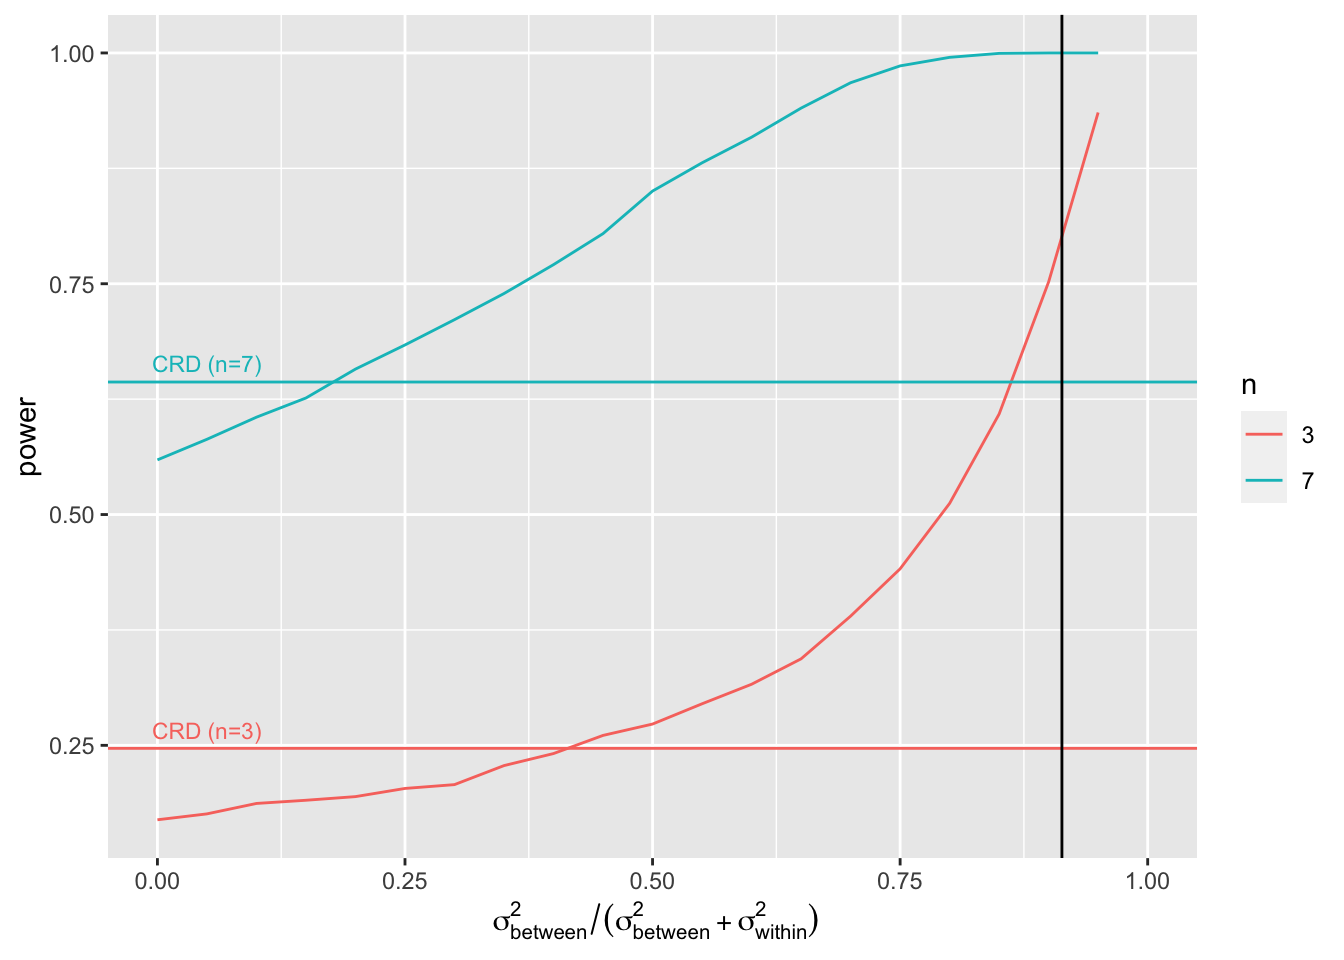
\includegraphics{experimentalDesignI_files/figure-latex/unnamed-chunk-25-1.pdf}

\end{document}
